% -*- mode: latex; -*-
\DocumentMetadata{pdfstandard=X-4p}
\documentclass[aspectratio=169,8pt]{beamer}
\usetheme{metropolis}

% Standard packages

\usepackage[english]{babel}
%\usepackage[latin1]{inputenc}
%\usepackage{times}
%\usepackage[T1]{fontenc}
\usepackage{fontspec}
\usepackage[]{unicode-math}
\setsansfont{Roboto}
\usepackage{amsmath}

% Setup asymptote
\usepackage[inline]{asymptote}

\newcounter{counter}
% Author, Title, etc.

\title{Graphs}

\author[Shiv Shankar Dayal]{Shiv Shankar Dayal}

\begin{document}
\begin{frame}
  \titlepage
\end{frame}
\begin{frame}{Applications of graphs}
  \begin{itemize}
  \item How to find fastest route between different cities of the world?
  \item How can $n$ jobs be given to $n$ people with maximum total utility?
  \item How to lay telephone network cables at minimum cost?
  \item How can a map be colored using four colors in such a way that neghboring regions receive different
    colors?
  \item How should a salesman travel so that he can minimize travel time when visiting different cities?
  \end{itemize}
\end{frame}
\begin{frame}{Few Graphs}
  \begin{center}
    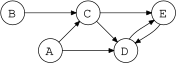
\includegraphics[scale=0.5]{graph}
  \end{center}
\end{frame}
\begin{frame}{Terminology}
  A graph consists of {\it nodes} or {\it vertices}. The set of vertices is called {\it vertex set} and is
  typically denoted by $V(G) = \{v_1, \ldots, v_n\}$, where $G$ is represents the graph.

  Nodes or vertices are connected by {\it arcs} or {\it edges}. The set of edges or arcs is called {\it edge set}
  and is typically denoted by $E(G) = \{e_1, \ldots, e_n\}$.

  In the diagram (a) shown $V(G) = \{A, B, C, D, E, F, G, H\}$ and $E(G) = \{(A, B), (A, C), (A, D), (C, D), (C, F),
  (E, G), (A, A)\}$.

  When the node pairs, of which, the edges constitute are ordered pairs, the graph is said to be a {\it directed
    graph} or {\it digraph}. Graphs shown (b), (c) and (d) are digraphs.

  The head of each arrow represents the second vertex of the ordered pair of vertices making up an edge, and the tail
  of each arrow represents the first vertex of the ordered pair.

  The edge set for the graph (b) is given by $E(G) = \{<A, B>, <A, C>, <A, D>, <C, D>, <F, C>, <E, G>, <A, A>\}$.

  Note that a graph is not always a tree, but a tree is always a graph. Also, a vertex need not have a connection
  mandatorily. As you can see in (a) node $H$ is on its own.
\end{frame}
\begin{frame}{Terminology Contd.}
  A vertex $v$ is incident to an edge $e$ if $v$ is one the two vertices in the ordered pair of vertices that
  constitute $e$. This is written as $u\leftrightarrow v$ to mean ``$u$ is adjacent to $v$''. Here $u$ is called
  {\it successor} of $v$ and $v$ is called {\it predecessor} of $u$.

  A {\it loop} is an edge whose endpoints are equal. For example, $<a, a>$ is a loop. {\it Parallel edges} or {\it
    multiple edges} are the edges that have same pair of endpoints. For example as shown in graph (d).

  If $n$ edges are incident on a vertex then that vertex has a {\it degree} of $n$. If a vertex has $n$ incoming
  edge then that is called {\it indegree} of the vertex and no. of outgoing edges are called {\it outdegree}.

  A {\it relation} $R$ on a set $A$ is a set of ordered pairs of elements of $A$.

  A graph in which edges have a number associated with them is called a {\it weighted graph} or a {\it network}
  and the number is called the {\it weight}.

  A path of length $l$ from vertex $a$ to vertex $b$ is defined as a sequence of $l + 1$ vertices
  $v_1, v_2, \ldots, v_{l + 1}$ such that $v_1 = a, v_{l + 1} = b$ and {\tt adjacent($v_i, v_i + 1$)} is {\tt true}
  for all $i$ between 1 and $l$. A path from a vertex to itself is called a {\it cycle} like vertex $A$ in (a).
  If a graph contains a cycle, it is {\it cyclic}m otherwise it is {\it acyclic}. A directed acyclic graph is
  called a dag from its acronym. For example, a git source tree is DAG.
\end{frame}
\begin{frame}{Warshall's Algorithm}
  Define ${\tt path_k[i][j]}$ to be {\tt true} if and only if there is a path from vertex {\tt i} to {\tt j}
  that does not pass through any vertices higher than {\tt k}(except for {\tt i} and {\tt j}).

  Clearly, if ${\tt path_k[i][j]}$ is {\tt true} then ${\tt path_{k + 1}[i][j]}$ will also be {\tt true}.
  However, if ${\tt path_k[i][j]}$ is {\tt false} then for ${\tt path_{k + 1}[i][j]}$ to be {\tt true} there
  has to be a path from {\tt i} to {\tt j} through {\tt k + 1} but there is no path from {\tt i} to {\tt j}
  through nodes {\tt 1} to {\tt k}. That is ${\tt path_k[i][k + 1] == true \&\& path_k[k + 1][j] == true}$.
\end{frame}
\begin{frame}{Adjacency List Representation}
  We have seen adjancency matrix representation of graphs. The main problem is that the memory consumption
  is very high for adjancency matrix representation. To reduce the memory consumption we have an alternative
  representation for graphs using linked lists which is known as adjacency list representation.
  \vspace*{0.5cm}
  An array/vector of lists stores edges between two vertices. Array's size is equal to the
  no. of vertices (i.e, {\tt n}). Each index represents a specific vertex in the graph. The
  entry at the index {\tt i} of the array points to a linked list containing the vertices that are adjacent to
  vertex {\tt i}.

  If there are {\tt n} vertices in the graph, then we create an array of list of same size as {\tt
    adj\_list[n]}.
\end{frame}
\begin{frame}[fragile]{Undirected graph to adjacency list}
  \begin{center}
    \begin{figure}
      \includegraphics{und-graph}
    \end{figure}
    \begin{figure}
      \includegraphics{und-adj-list}
    \end{figure}
  \end{center}
\end{frame}
\begin{frame}[fragile]{Directed graph to adjacency list}
  \begin{center}
    \begin{figure}
      \includegraphics{di-graph}
    \end{figure}
    \begin{figure}
      \includegraphics{di-adj-list}
    \end{figure}
  \end{center}
\end{frame}
\begin{frame}[fragile]{Breadth First Search}
  \begin{center}
    \begin{figure}
      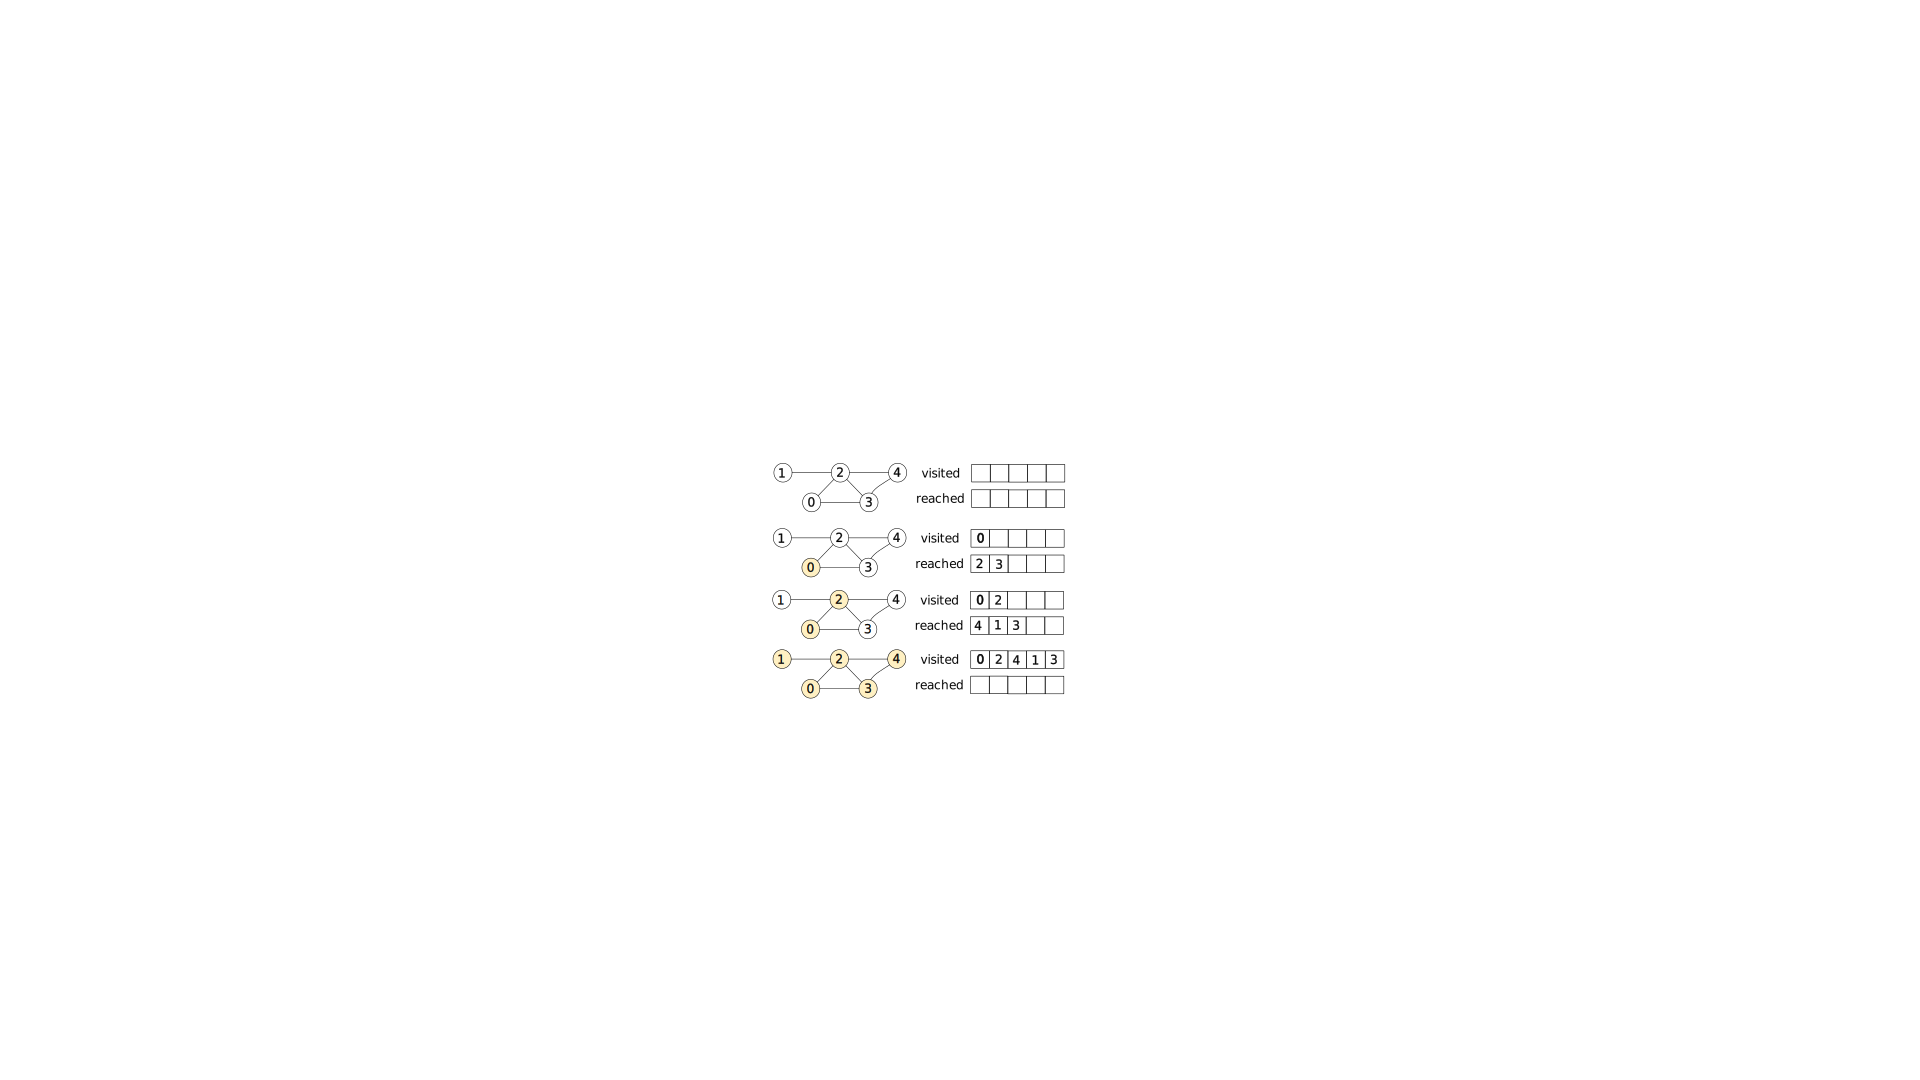
\includegraphics{bfs}
    \end{figure}
  \end{center}
\end{frame}
\begin{frame}[fragile]{Depth First Search}
  \begin{center}
    \begin{figure}
      \includegraphics{dfs}
    \end{figure}
  \end{center}
\end{frame}
\begin{frame}{Properties of search algorithms}
  \begin{itemize}
  \item {\bf Time Complexity:} How much time does the algorithm take?
  \item {\bf Space Complexity} How much memory does the algorithm consume?
  \item {\bf Completeness:} Is the algorithm guaranteed to find a solution when there is one, and
    to correctly report failure when there is not?
  \item {\bf Cost optimality:} Does it find a solution with the lowest path cost of all solutions?
  \end{itemize}

  BFS is complete if {\tt b} is finite, and the state space either has a solution or is finite
  and cost-optimal if action costs are all identical. $b$ is the branching factor or number of
  successors of a node that need to be considered.
\end{frame}
\begin{frame}{Dijkstra's Shortest Path Algorithm}
  \begin{itemize}
  \item Create a shotest path tree set that tracks the vertices in the shortest path tree. It is empty
    to begin with.
  \item Assign distance values to all vertices in the graph. Initially distance values are infinite
    except the distance of source from itself which is initiallized to 0.
  \item while shortest path tree does not include all vertices
    \begin{itemize}
    \item Pick a vertex {\tt u} that is not there in shortest path tree and has a minimum distance value and
      include it to shortest path tree
    \item Update the distance value of all adjacent vertices of {\tt u}
    \item For every adjacent vertex {\tt v}, if the sum of distance value of {\tt u} from source and weight
      of the edge {\tt u-v} is less than the distance value of {\tt v}, then update the distance value of
      {\tt v}.
    \end{itemize}
  \end{itemize}
\end{frame}
\begin{frame}[fragile]{Dijkstra's Shortest Path Algorithm}
  \begin{center}
    \begin{figure}
	    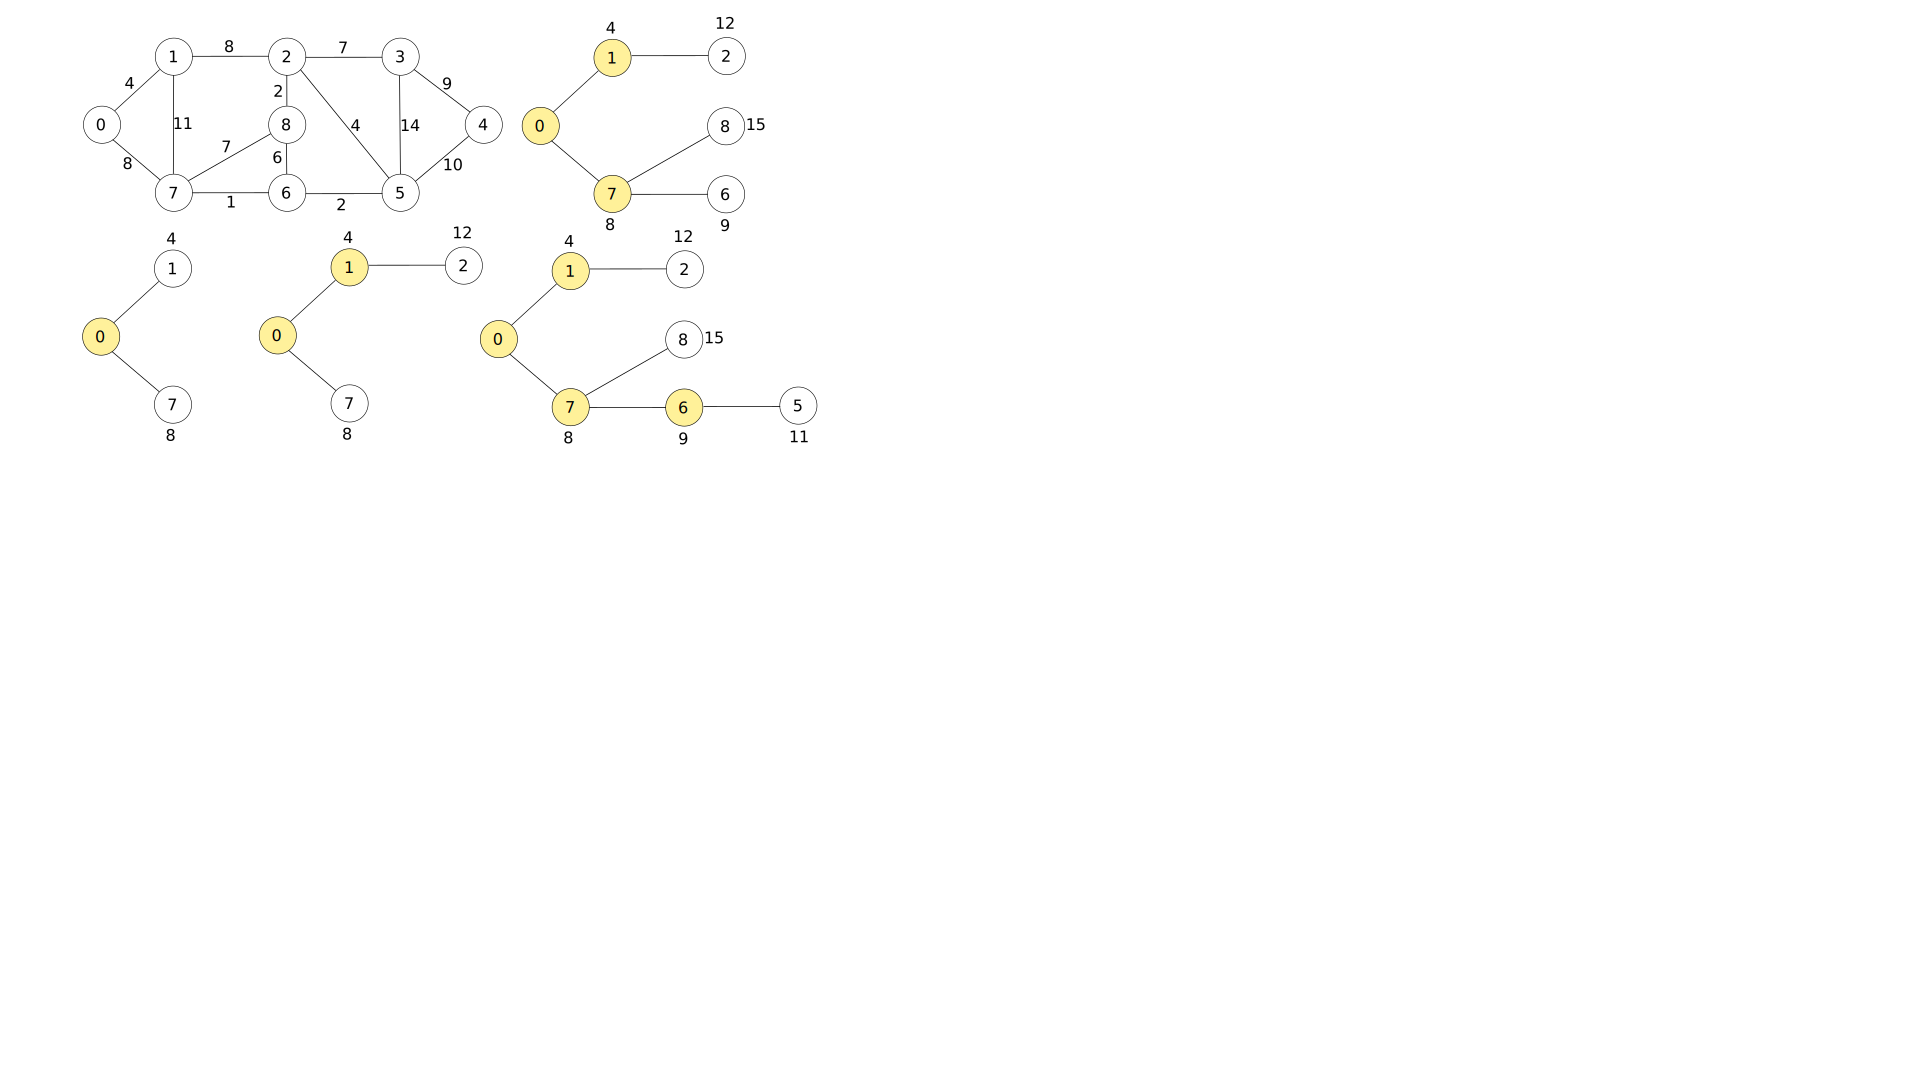
\includegraphics[height=60mm]{dijkstra}
    \end{figure}
  \end{center}
\end{frame}
\end{document}
